\section{Aufbau der Stoffe}

\subsection{Bindungsarten}
\begin{itemize}
	\item Kovalente Bindung (Atombindung)
		\begin{itemize}
			\item 2 nichtmetallische Atome
			\item Moleküle, Makromoleküle oder Atomgitter
		\end{itemize}
	\item Ionenbindung
		\begin{itemize}
			\item Elektrostatische Anziehung zwischen pos. (Kation) und neg. (Anion) geladenem Ion
			\item Ionengitter (Salze)
		\end{itemize}
	\item Metallbindung
		\begin{itemize}
			\item Elektrostatische Anziehung zwischen metallischen Kation und delokalisierten Elektronen
			\item Kationengitter (Metalle und Legierungen)
		\end{itemize}
\end{itemize}

\subsection{Stoffklassen}
\begin{itemize}
	\item Flüchtige Stoffe (molekulare Stoffe und Edelgase)
	\begin{itemize}
	    \item \textbf{Eigenschaften:} tiefe Schmelz- und Siedetemperatur, nicht leitend, weich
	    \item \textbf{Aufbau:} Molekül (abgeschlossener Atomverband aus Nichtmetallatomen), Edelgase kommen atomar vor
	    \item \textbf{Bindungsart:} Atombindung, gemeinsames Elektronenpaar zw. neutralen Nichtmetallatomen
	    \item \textbf{Beispiel:} $CO_2$, $I_2$, $CH_3CH_2OH$
	\end{itemize}
	\item Salzartige Stoffe
	\begin{itemize}
	    \item \textbf{Eigenschaften:} hohe Schmelz- und Siedetemperatur, im flüssigen oder gelösten Zustand leitend, als Feststoff hart und spröde
	    \item \textbf{Aufbau:} bestehen aus Ionen, die ein unendlich grosses 3-dimensionales Gitter bilden
	    \item \textbf{Bindungsart:} Ionenbindung, elektrostatische Anziehung (Coulomb-Kraft) zwischen Kationen und Anionen
	    \item \textbf{Beispiel:} $CaCO_3$, $CaSO_4$, $Na_2CO_3$
	\end{itemize}
	\item Metallische Stoffe
	\begin{itemize}
	    \item \textbf{Eigenschaften:} elektrisch leitend, metallischer Glanz, häufig hohe Schmelz- und Siedetemperaturen, verformbar (duktil), gute Wärmeleiter
	    \item \textbf{Aufbau:} Metallkationen, die ein unendlich grosses 3-dimensionales Gitter bilden, sind von Elektronengas umgeben
	    \item \textbf{Bindungsart:} Metallbindung, elektrostatische Anziehung (Coulomb-Kraft) zwischen Kationen und Elektronengas
	    \item \textbf{Beispiel:} Metalle und Legierungen (Messing, Stahl, Amalgam)
	\end{itemize}
	\item Hochmolekulare Stoffe (Polymere)
	\begin{itemize}
	    \item \textbf{Eigenschaften:} sehr hart, sehr hohe Schmelz- und Siedetemperatur, nicht leitend
	    \item \textbf{Aufbau:} Atomgitter, die sowohl Nichtmetall- als auch Metallatome enthalten können
	    \item \textbf{Bindungsart:} Atombindung, Ionenbindung
	    \item \textbf{Beispiel:} $C$, $SiO_2$, $Al_2O_3$
	\end{itemize}
	\item Diamantartige Stoffe
	\begin{itemize}
	    \item \textbf{Eigenschaften:} keine definierte Schmelztemperatur sondern allmähliches Erweichen, kein Verdampfen sondern Zersetzung
	    \item \textbf{Aufbau:} sehr lange Moleküle, die aus Atomgruppen (Monomeren) bestehen
	    \item \textbf{Bindungsart:} Atombindung
	    \item \textbf{Beispiel:} Kunstoffe (Nylon, PVC, PET, Silikon), natürliche Polymere (Eiweiss, Stärke, DNA)
	\end{itemize}
\end{itemize}

\subsection{Stoffmengen und Stoffmassen}
$1$ $mol$ entsprechen $6.02 \cdot 10^{23}$ Stoffteilchen. Die Zahl $6.02 \cdot 10^{23}$ wird als Avogadro-Zahl $N_A$ bezeichnet.

\subsubsection{Molare Masse}
Die molare Masse $M$ ist die Masse von $1$ $mol$ eines Stoffes. \\
$M=\frac{m}{n}$ \ \ $[M]=\frac{g}{mol}$

\subsection{Kristallstrukturen}
\begin{itemize}
	\item Kristalline Feststoffe (regelmässige Anordnung = Fernordnung), z.B. Metalle, Salze, diamantartige
	\item Amorphe Feststoffe (unregelmässige Anordnung = Nahordnung), z.B. Kunststoffe, Glas
\end{itemize}

\subsubsection{Das Harte-Kugeln-Modell}
\begin{figure}[htbp]
	\begin{subfigure}{0.49\linewidth}
		\centering
		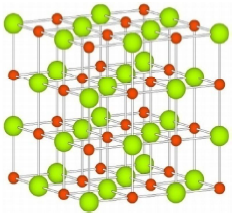
\includegraphics[width=0.49\linewidth]{images/1_Raumgittermodell.png}
		\caption{Raumgittermodell}
	\end{subfigure}
	\begin{subfigure}{0.49\linewidth}
		\centering
		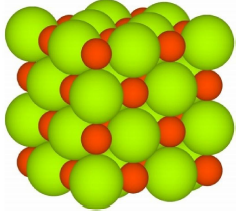
\includegraphics[width=0.49\linewidth]{images/1_Kugelpackungsmodell.png}
		\caption{Kugelpackungsmodell}
	\end{subfigure}
\end{figure}

\subsection{Dichteste Kugelpackungen}
\begin{figure}[htbp]
	\begin{subfigure}{0.49\linewidth}
		\centering
		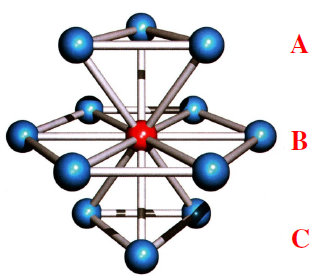
\includegraphics[width=0.49\linewidth]{images/1_kubisch_dichteste_KuPa.png}
		\caption{Kubisch dichteste Kugelpackung}
	\end{subfigure}
	\begin{subfigure}{0.49\linewidth}
		\centering
		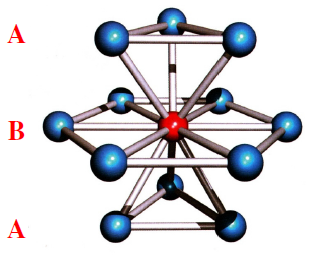
\includegraphics[width=0.49\linewidth]{images/1_hexagonal_dichteste_KuPa.png}
		\caption{Hexagonal dichteste Kugelpackung}
	\end{subfigure}
\end{figure}

\subsubsection{Lücken}
\begin{itemize}
	\item Oktaederlücken: oktaedrisch von 6 Atomen umgeben
	\item Tetraederlücken: tetraedrisch von 4 Atomen umgeben
	\item Koordinationszahl (KZ): Zahl der nächsten Nachbarteilchen (12 bei  dichtester Kugelpackung)
\end{itemize}

\subsection{Elementarzelle}
Kleinste Einheit einer Kristallstruktur. Erlaubt eindeutige Beschreibung des atomaren Aufbaus. 

\begin{multicols}{2}
    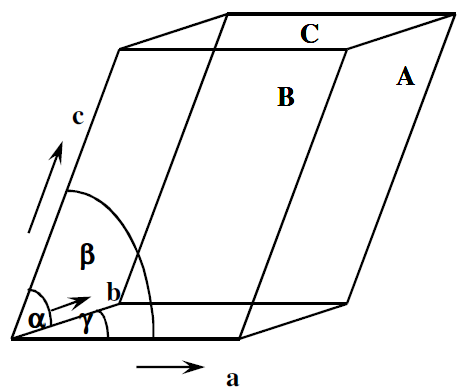
\includegraphics[width=2.5cm]{images/1_Elementarzelle.png}
    
\columnbreak

    Durch 6 Gitterparameter $a$, $b$, $c$, $\alpha$, $\beta$, $\gamma$ eindeutig bestimmt. Es existieren 14 Arten von Elementarzellen. Die drei häufigsten sind: \\
\end{multicols}

\begin{figure}[htbp]
	\begin{subfigure}{0.32\linewidth}
		\centering
		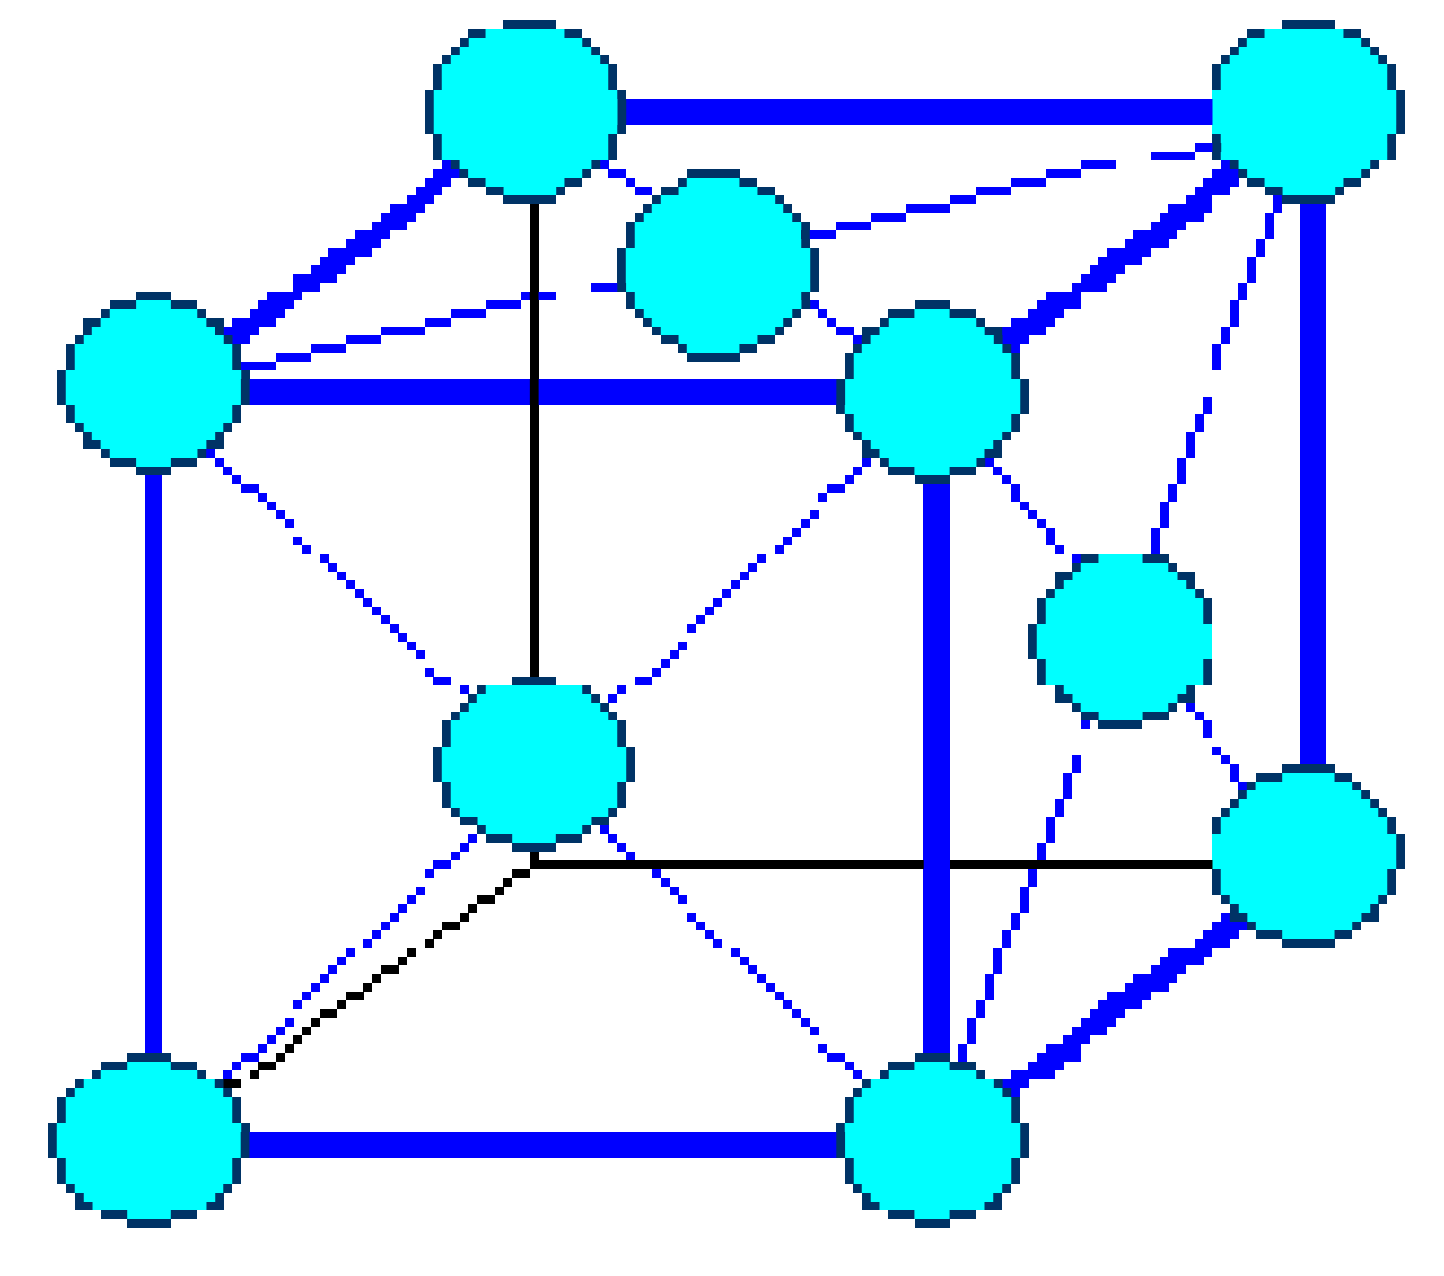
\includegraphics[width=0.5\linewidth]{images/1_kfz.png}
		\caption{kubisch flächenzentriert}
	\end{subfigure}
	\begin{subfigure}{0.32\linewidth}
		\centering
		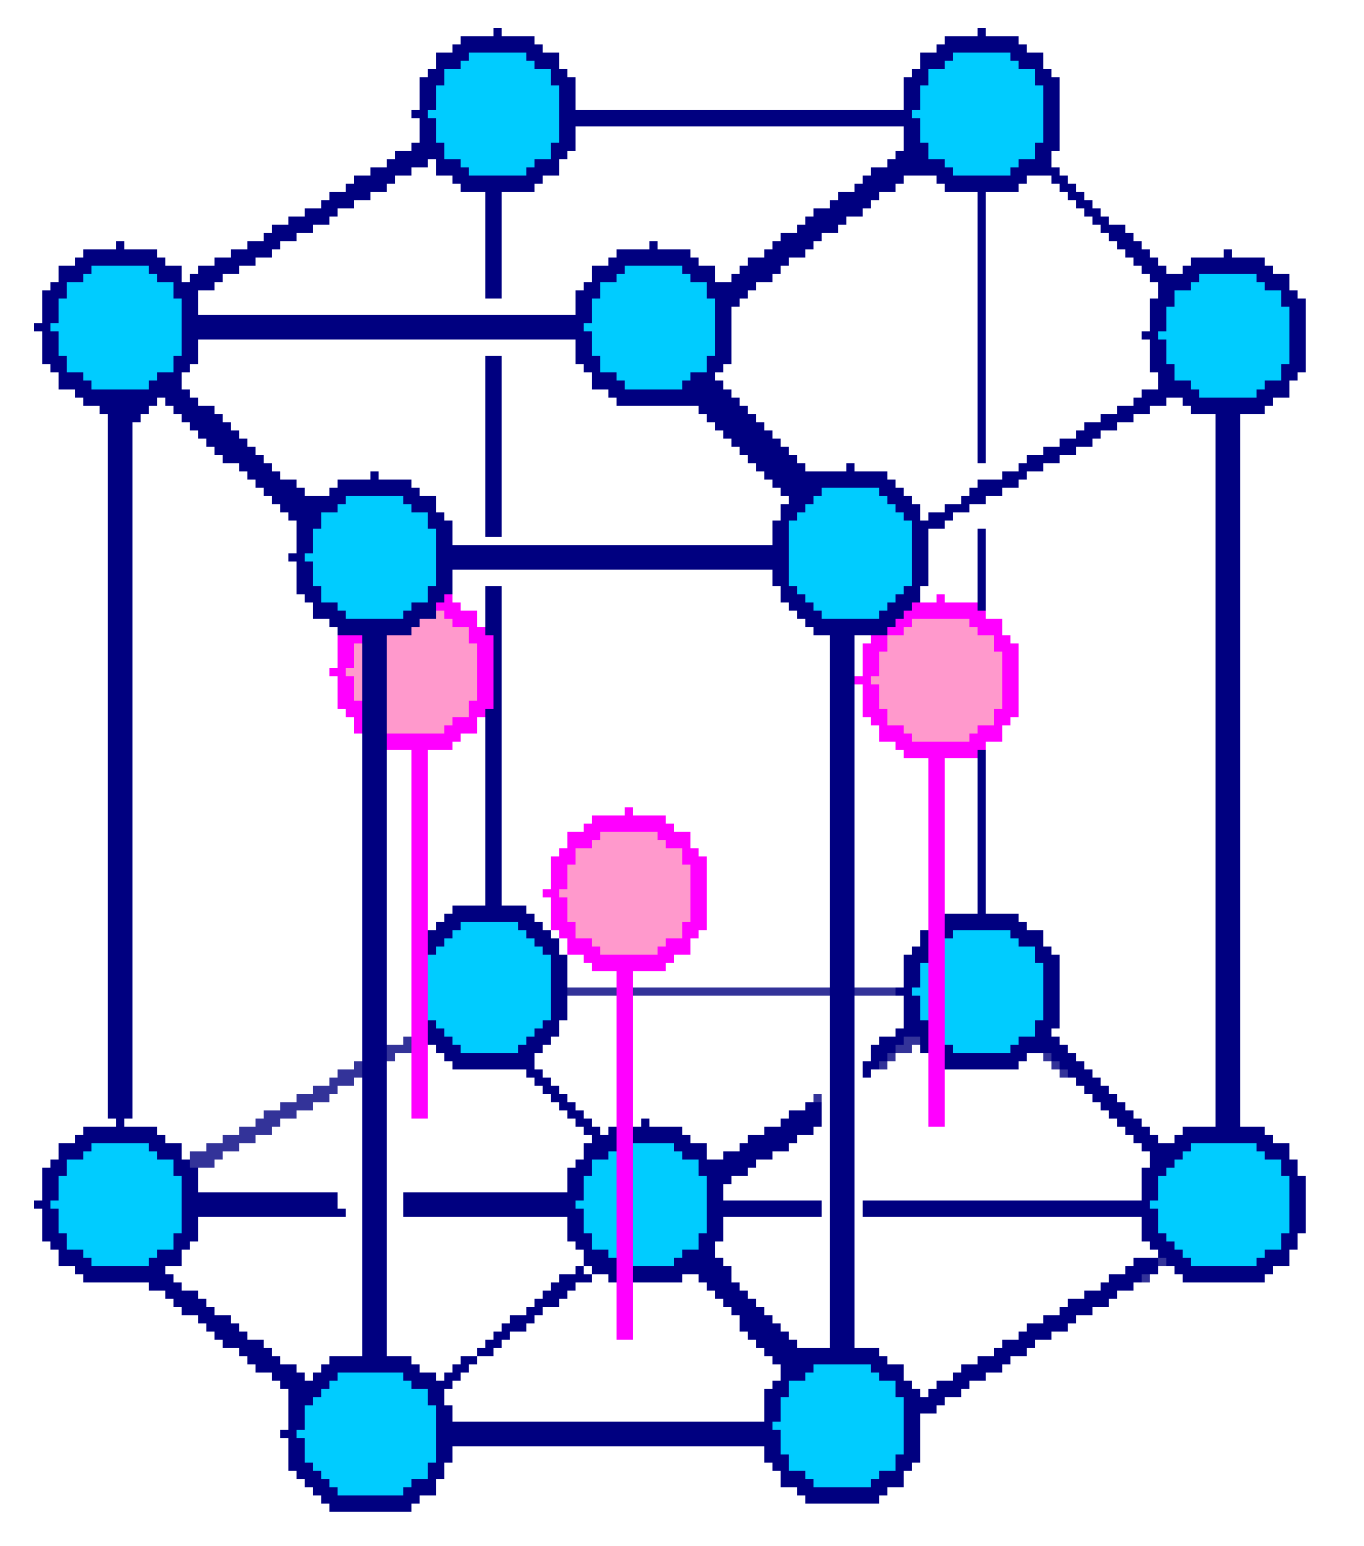
\includegraphics[width=0.5\linewidth]{images/1_hcp.png}
		\caption{hexagonal dichtest gepackt}
	\end{subfigure}
	\begin{subfigure}{0.32\linewidth}
		\centering
		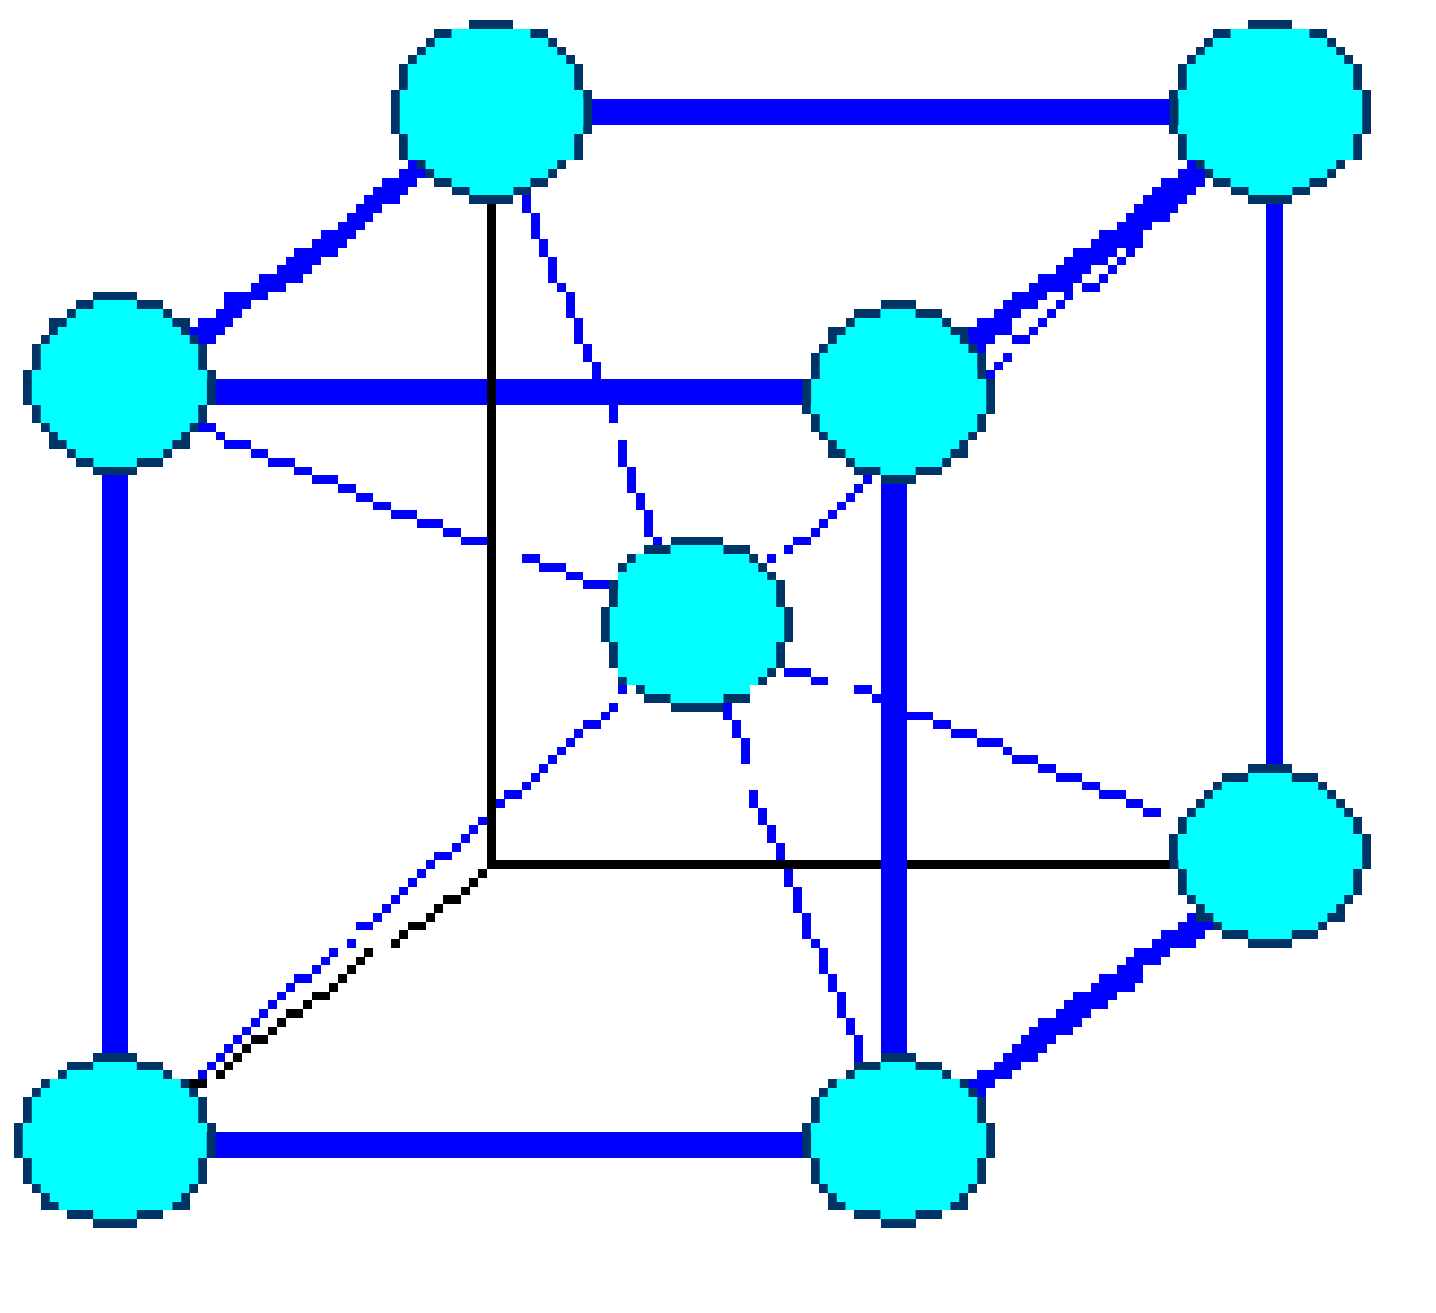
\includegraphics[width=0.5\linewidth]{images/1_krz.png}
		\caption{kubisch raumzentriert}
	\end{subfigure}
\end{figure}

\subsection{Packungsdichte}
Packungsdichte $P = \frac{V_{Atome}}{V_{Elementarzelle}}$, Raumerfüllung durch Atome einer Elementarzelle. Für dichteste Kugelpackungen ist $P=74\%$

\subsection{Gitterfehler}
\begin{itemize}
	\item Versetzung
	\item Unbesetzter Gitterplatz
	\item Fremdatom in Gitterlücke
	\item Fremdatom in Gitterplatz
\end{itemize}